\section{Skill Acquisition}\label{sec:skillacquisition}

This section analyzes endogenous skill acquisition. We find that equilibrium multiplicity at the trading stage leads to middling skill investments and reveals the potential for multiplicity in the optimal skill levels.

\subsection{Setup}
Before the trading stage in $t=0$, each trader makes a costly investment to improve her skill potential. This investment could include pursuing an advanced degree in finance, studying for professional exams, or engaging in specialized training to expand her expertise. The trader selects her skill potential, denoted as $\omega_{s}^{*}$, by paying the skill-acquisition cost, $C(\omega_{s}^*) = c\omega_{s}^{*}$ with a positive marginal cost $c>0$.\footnote{The following analysis does not hinge on the functional form of the cost, as long as it is weakly increasing in $\omega_{s}^{*}$.} We assume that $\omega_{s}^{*}$ is not observable to the market makers and the recruiter. Instead, they form a belief about it, denoted by $\omega_{s}$, and the equilibrium in the trading stage is determined by $\omega_{s}$ following Proposition \ref{prop:endogenous}. On the equilibrium path, the belief must be consistent with the actual skill potential, $\omega_{s}^{*} = \omega_{s}$. However, at the skill-acquisition stage, the trader cannot influence $\omega_{s}$, as she does not have a commitment device.\footnote{This setting follows the literature on private information acquisition with an unobservable quality (precision) of the private signal. See, for example, \citet{xiong2023secret}.}

\paragraph{\normalfont{\it{Expected utility of a trader.}}}
Given the realized equilibrium in the first trading stage (i.e., $\beta_{0}$), the \textit{ex-ante} expected utility of a trader is characterized by the following lemma:
\begin{lemma}\label{lem:expU_skill}
For each $\beta_{0}$, the expected utility of a trader at the skill-acquisition stage is given by
\begin{equation}
 V(\omega_{s}^{*},\omega_{s},\beta_{0}) = v(\omega_{s},\beta_{0})\omega_{s}^{*} + \bar{v}, \label{eq:exanteV}
\end{equation}
where $\bar{v}$ summarizes constant terms unrelated to $\omega_{s}^{*}$,\footnote{The formal expression is given by $\bar{v} =\frac{\psi}{4\lambda_{1}}\left[{\xi}^{2}\gamma^{2}\omega_{u,0}+\xi^{2}(1-\gamma)^{2}\omega_{\delta}+\omega_{u,0}\frac{\gamma\xi}{\beta_{0}}\right]$} and $v(\omega_{s},\beta_{0})$ is
\begin{align}
     v(\omega_{s},\beta_{0})\equiv&(1-\lambda_{0}\beta_{0})\beta_{0}   +(1-\psi)\frac{1}{2}\sqrt{\frac{\omega_{u,1}}{\omega_{s}}} \nonumber \\
     & +\theta \xi^2 \left[\gamma^2 \beta_{0}^2 + 2\gamma(1-\gamma)\beta_{0}+ (1-\gamma)^2\right].\label{eq:v_sbeta}
\end{align}
\end{lemma}

Equation (\ref{eq:exanteV}) indicates that, for each unit of the selected skill potential ($\omega_{s}^{*}$), the trader earns the marginal utility of $v(\omega_{s},\beta_{0})$.
The marginal utility in equation (\ref{eq:v_sbeta}), in turn, consists of three factors. The first two terms represent the maximized trading profit in $t=0$ and that in $t=1$ when she does not meet the recruiter. In the first trading round, the equilibrium profit margin of the skill potential is $(1-\lambda_{0}\beta_{0})\beta_{0}$, while the profit margin in the second trading round is identical to that in the standard \cite{kyle1985continuous} model.\footnote{In the standard \citet{kyle1985continuous} model, the optimal trading intensity is $\beta_{0} = \frac{1}{2\lambda_{0}}$, so that the equilibrium profit margin of the information advantage (i.e., the skill in our model) is directly captured by $\frac{\beta_{0}}{2}$. Our model does not have this feature, as the trading intensity is set by incorporating both the price impact and the reputation concern.} The third term is the reaction of the reputation benefit to an increase in the selected skill potential, which emanates from the reputation concerns, $\theta$, and the magnitude of the recruiter's belief updating (see equations [\ref{etahat_b}] and [\ref{w}]).  

Importantly, $v(\omega_{s},\beta_{0})$ is characterized by the market's belief about the trader's skill potential ($\omega_{s}$), as $\omega_{s}^{*}$ is unobservable to the market. The trader cannot influence $\omega_{s}$ by controlling $\omega_{s}^{*}$ due to limited commitment. Consequently, the optimality condition for the skill acquisition is characterized by $\omega_{s}$, as the following discussion elaborates.

\paragraph{\normalfont{\it{Sunspot shock.}}}
To formalize the skill-acquisitiom problem based on Lemma \ref{lem:expU_skill}, we introduce an equilibrium-selection device. In particular, following the most common approach, we assume that market participants condition their actions on the realization of an exogenous \textit{sunspot} shock, characterized by the binary random variable $z\in\{0,1\}$.\footnote{The sunspot equilibrium is proposed by \citet{diamond1983bank} as an equilibrium selection device in the context of bunk runs and formalized in the equilibrium analyses by the subsequent studies, such as \citet{cooper1998bank}.} Namely, when $\omega_{s}\in (\ubar{\omega}_{s},\bar{\omega}_{s})$, they play the high-$\beta$ equilibrium if a spot appears on the sun ($z=1$), whereas the low-$\beta$ equilibrium is realized if no spots are observed ($z=0$). Accordingly, the high-$\beta$ equilibrium is realized with probability $\Pr(z=1)=\rho$, where $\rho$ denotes the exogenous probability of a sunspot. We assume that $z$ is realized at the beginning of the trading stage in $t=0$, meaning that a trader acquires her skill potential before $z$ is realized. In what follows, the high-$\beta$ and low-$\beta$ equilibria are denoted as $\beta_{0} = \beta_{H}$ and $\beta_{L}$, respectively.

By incorporating the equilibrium multiplicity stipulated in Proposition \ref{prop:endogenous}, the trader's \textit{ex-ante} expected utility from acquiring $\omega_{s}^{*}$ in equation (\ref{eq:exanteV}) is rewritten as follows:\footnote{We omit the constant term, $\bar{v}$, in the following discussion, as it does not affect the optimal skill potential.}
\begin{equation}
\mathrm{E}_{\beta}[v(\omega_{s},\beta_{0})]\omega_{s}^{*}  = 
\begin{cases}
v(\omega_{s},\beta_{L}) \omega_{s}^{*} & \text{if } \omega_{s} \geq \bar{\omega}_{s}, \\
\left[\rho v(\omega_{s},\beta_{H}) + (1-\rho) v(\omega_{s},\beta_{L})\right]\omega_{s}^{*} & \text{if } \omega_{s} \in (\ubar{\omega}_{s}, \bar{\omega}_{s}), \\
v(\omega_{s},\beta_{H}) \omega_{s}^{*} & \text{if } \omega_{s} \leq \ubar{\omega}_{s}.
\end{cases}
\label{eq:barV_2}
\end{equation}
$\mathrm{E}_{\beta}$ denotes the expectation over  $\beta_{0} = \beta_{H}$ and $\beta_{L}$ in cases of multiple equilibria and incorporates the sunspot shock with $\rho = \Pr(z=1) = \Pr(\beta_{0}=\beta_{H})$. 

\subsection{Equilibrium}

Prior to the trading game, each trader solves the following problem by controlling her skill potential:
\begin{equation}
\max_{\omega_{s}^{*}} \mathrm{E}_{\beta}[v(\omega_{s},\beta_{0})]\omega_{s}^{*} - C(\omega_{s}^{*}), \label{eq:skillacquisition}
\end{equation}
where $\mathrm{E}_{\beta}[v(\omega_{s},\beta_{0})]\omega_{s}^{*}$ is given by equation (\ref{eq:barV_2}). As the trader cannot control $\omega_{s}$, she takes the marginal benefit in (\ref{eq:barV_2}) as given. 

In the equilibrium, the marginal benefit balances the marginal cost of skill acquisition, as equation (\ref{eq:FOC_SA}) below illustrates. Otherwise, the trader has an incentive to increase or decrease $\omega_{s}^{*}$. Together with the belief-consistency condition, the optimal skill potential $\omega_{s}^{*}$ is derived as solutions to the following optimality condition with respect to $\omega_{s}$:
\begin{equation}
\mathrm{E}_{\beta}[v(\omega_{s},\beta_{0})] = c.\label{eq:FOC_SA}
\end{equation}

\begin{figure}[t]
\centering
{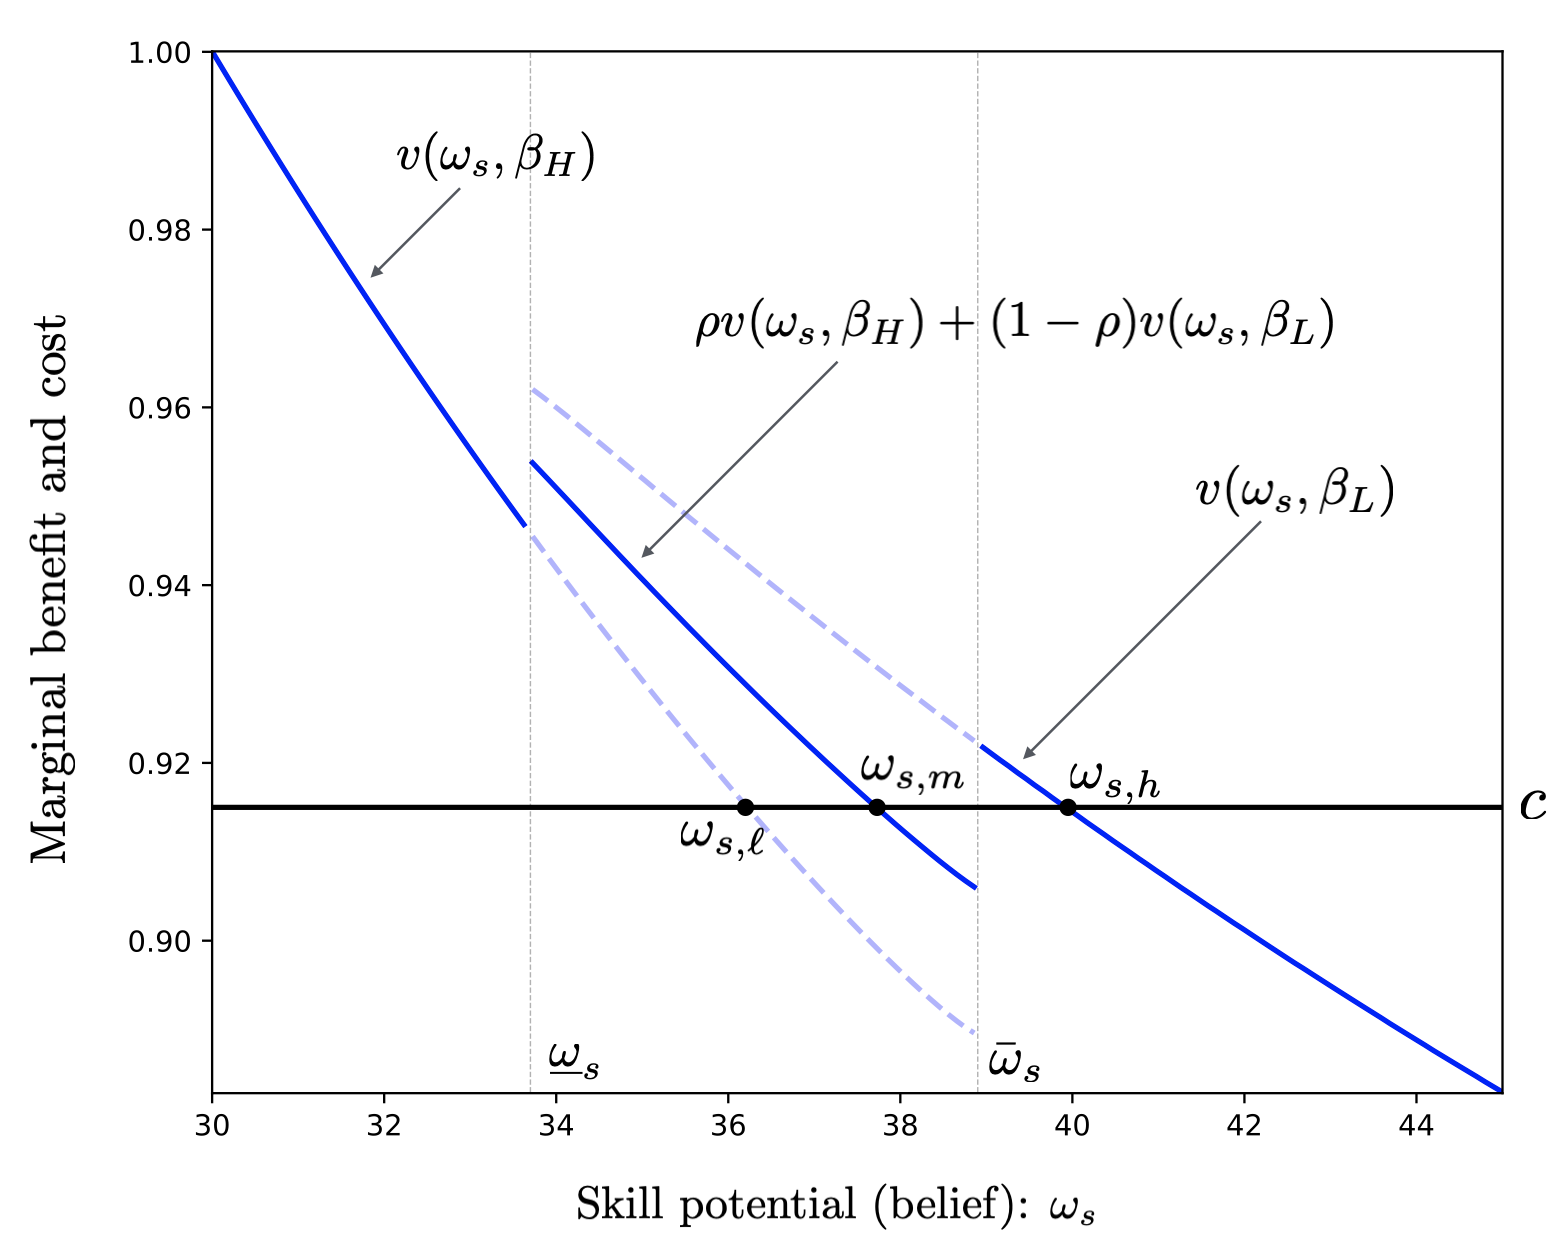
\includegraphics[width=99mm]{./Figures/skillpotential.png}}\\[10pt]
\caption{Marginal Benefit and Cost of Skill Acquisition}
\caption*{\footnotesize{Note: The figure plots the marginal benefit of skill acquisition, given by $\mathrm{E}_{\beta}[v(\omega_{s},\beta_{0})]$, and its marginal cost $c$ against the belief about the skill potential, $\omega_{s}$. The parameter values are $\omega_{\delta}=1$, $\omega_{u,0}=0.1$, $\omega_{u,1}=60$, $\theta=\frac{\varphi\beta_1}{2}\approx0.33$ ($\varphi=0.6$), and $\rho = 0.5$.}}\label{fig:skill_potential}
\end{figure}

Figure \ref{fig:skill_potential} plots the marginal benefit (the LHS of [\ref{eq:FOC_SA}]) in relation to the market's belief about the skill potential, $\omega_{s}$. Although it is orthogonal to the actual skill potential, $\omega_{s}$ and $\omega_{s}^{*}$ on the equilibrium path are determined by the intersections of the marginal benefit and the marginal cost curves in Figure \ref{fig:skill_potential}. 

%The marginal benefit of skill acquisition globally diminishes as $\omega_{s}$ increases. Intuitively, when the market maker believes that the trader has acquired a high skill potential, the price impact grows, and the trading intensity diminishes in both trading rounds at $t=0$ and $t=1$, thereby reducing the value of the skill. Conversely, when $\omega_{s}$ is high, the recruiter faces higher prior uncertainty in estimating the realized skill ($|s|$), and the wage becomes more reliant on the price information ($p_{0}$) and the asset payoff in $t=0$ ($\delta_{0}$). Hence, the wage becomes more sensitive to the trader's skill, making it more valuable for the trader to acquire a higher skill potential. Although the second channel encourages the trader to increase $\omega_{s}^{*}$, the first negative effect is dominant, forming the downward-sloping marginal benefit curve in Figure \ref{fig:skill_potential}.

The marginal benefit of skill acquisition globally diminishes as $\omega_{s}$ increases. This result is not obvious because there are two channels through which $\omega_{s}$ affects its marginal benefit. In the first channel, when the market maker believes that the trader has acquired a high $\omega_{s}$, the price impact grows, and the trading intensity diminishes in both trading rounds at $t=0$ and $t=1$, thereby reducing the benefit of increasing $\omega_{s}^{\ast}$. Conversely, in the second channel, when $\omega_{s}$ is high, the recruiter faces higher prior uncertainty in estimating the realized skill ($|s|$), and the wage becomes more reliant on the price information ($p_{0}$) and the asset payoff in $t=0$ ($\delta_{0}$). Hence, the wage becomes more sensitive to the trader's skill, making it more valuable for the trader to acquire a higher skill potential $\omega_{s}^{\ast}$. Although the second channel encourages the trader to increase $\omega_{s}^{*}$, the negative effect in the first channel is dominant, forming the downward-sloping marginal benefit curve in Figure \ref{fig:skill_potential}.

Notably, the marginal benefit curve in the skill-acquisition stage has discontinuities due to the multiple equilibria in the trading stage. When the (belief of) skill potential is sufficiently high or low ($\omega_{s}\geq \bar{\omega}_{s}$ or $\omega_{s}\leq \ubar{\omega}_{s}$), $\beta_{0}$ in the trading stage is uniquely determined. However, when the skill potential turns to intermediate levels, the trader starts incorporating the possibility of multiple equilibria in the trading stage, generating jumps in the marginal benefit of skill acquisition. By focusing on the intermediate levels of $\omega_{s}\in(\ubar{\omega}_{s},\bar{\omega}_{s})$, we obtain the following result.
\begin{lemma}\label{lem:MB_beta}
With $\omega_{s}$ being fixed, the marginal benefit of increasing the skill potential is smaller in the high-$\beta$ equilibrium than in the low-$\beta$ equilibrium. Therefore, the following inequalities hold, and the marginal benefit curve has discontinuities at $\omega_{s}=\ubar{\omega}_{s}$ and $\omega_{s}=\bar{\omega}_{s}$:
\begin{equation}
v(\omega_{s},\beta_{H}) < \mathrm{E}_{\beta}[v(\omega_{s},\beta_{0})] < v(\omega_{s},\beta_{L}). \label{eq:v_beta}
\end{equation}
\end{lemma}

Intuitively, the trader in the high-$\beta$ equilibrium excessively reveals information to the market
maker by trading aggressively. Although the recruiter estimates the trader's skill more precisely and increases the wage's sensitivity to the skill potential, it is dominated by the negative impact of a reduction in the trading profit margin. Therefore, the marginal benefit of increasing the skill potential becomes smaller in the high-$\beta$ equilibrium than in the low-$\beta$ equilibrium, leading to inequalities (\ref{eq:v_beta}). In what follows, we elaborate on the discontinuities and derive their implications for skill acquisition. 

\subsubsection{Middling Skill Acquisition}
We first propose ``middling" skill acquisition due to the multiple trading-stage equilibria by focusing on $\omega_{s}\in (\ubar{\omega}_{s},\bar{\omega}_{s})$. We refer to it as middling because the acquired skill level is either higher or lower than what she would acquire if she knew which type of equilibrium would be realized. On the equilibrium path, both the selected skill potential ($\omega_{s}^{*}$) and the market's belief about it ($\omega_{s}$) fall in this region if the marginal skill-acquisition cost is intermediate. In this region, the trading stage involves multiple equilibria (i.e., $\beta_{0} = \beta_{H}$ or $\beta_{L}$), whereas the trader at the skill-acquisition stage cannot influence the equilibrium selection.
%\footnote{The equilibrium realization in the trading stage is governed by the market's belief about the skill potential, $\omega_{s}$, as illustrated in Proposition \ref{prop:endogenous}, whereas the trader cannot influence it by selecting $\omega_{s}^{*}$ due to the lack of a commitment device.} 
Consequently, she determines her skill potential by anticipating the sunspot shock, which leads to the skill acquisition as follows. 
%We refer to it as \textit{conservative} because the acquired skill potential becomes either too high or too low compared to the skill potential she would acquire if she were allowed to select it again after the trading-stage equilibrium is realized.

%\begin{proposition}[Middling skill acquisition]\label{prop:skill_inef}
%The equilibrium skill potential in the presence of multiple trading-stage equilibria is middling in the sense that; 
%\begin{enumerate}[label=(\roman*)]
%\item It is lower than the skill potential that she would acquire in the low-$\beta$ equilibrium; and 
%\item It is higher than the skill potential that she would acquire in the high-$\beta$ equilibrium.
%\end{enumerate}
%\end{proposition}

\begin{proposition}[Middling skill acquisition]\label{prop:skill_inef}
The equilibrium skill potential in the presence of multiple trading-stage equilibria is
\begin{enumerate}[label=(\roman*)]
\item lower than the skill potential that she would acquire in the low-$\beta$ equilibrium; and 
\item higher than the skill potential that she would acquire in the high-$\beta$ equilibrium.
\end{enumerate}
\end{proposition}

Figure \ref{fig:skill_potential} illustrates a numerical example; $\omega_{s,m}$ is the ex-ante optimal skill potential, while the ex-post equilibrium is either $\omega_{s,\ell}$ or $\omega_{s,h}$, depending on the equilibrium
realization in the trading stage.

The trader invests in skill potential incorporating the possibility of both high- and low-$\beta$ equilibria. At the trading 
stage, however, the acquired skill potential turns out to be insufficient if the low-$\beta$ equilibrium is realized, as its optimal play involves the profit-driven strategy and requires a relatively high asset-selection skill (i.e., $\omega_{s,h}$ is the \textit{ex-post} equilibrium). Conversely, the acquired skill potential is too high if the high-$\beta$ equilibrium is realized, as the trader takes the reputation-driven strategy that does not require a high skill potential (i.e., $\omega_{s,\ell}$ is the \textit{ex-post} equilibrium). 

This result indicates that individuals or firms may invest in skills that seem oddly intermediate or cautious—neither fully specialized nor overly basic. For example, it explains why some traders and finance professionals choose to pursue broader business qualifications instead of more specialized academic paths, allowing them to adapt to a wide range of market situations. Traders also learn intermediate-level coding (e.g., Python) for algorithmic trading or data analysis but stop short of deep computer science expertise. A similar trend can be observed with respect to CFA Levels and quantitative skills among hedge fund managers. These skill acquisitions would be difficult to rationalize in an economy with a single equilibrium but become logical under the equilibrium multiplicity and uncertainty regarding equilibrium realization. 

\subsubsection{Fragile Skill Acquisition and Skill Diversity}
By expanding our scope to the entire range of skill potential ($\omega_{s}$), the discontinuities in Lemma \ref{lem:MB_beta} imply that the skill-acquisition problem in (\ref{eq:skillacquisition}) may have multiple solutions.\footnote{Although the equilibrium multiplicity in the trading stage (i.e., $\beta_{0}$) is determined by the level of $\omega_{s}$, as Proposition \ref{prop:endogenous} stipulates, it is orthogonal to the existence of multiple solutions to the optimal skill acquisition in equation (\ref{eq:FOC_SA}).} 

For example, when the marginal cost of skill acquisition is moderately small, as Figure \ref{fig:skill_potential} illustrates, both the high skill potential ($\omega_{s,h}$) and the intermediate skill potential ($\omega_{s,m}$) become optimal for the trader. Corresponding to $\omega_{s,h}$, the equilibrium in the trading stage is unique with $\beta_{0}=\beta_{L}$, where the trader engages in solid profit-driven trading. Conversely, the trading stage with skill potential $\omega_{s,m}$ involves multiple equilibria, and the selected skill potential is middling, as Proposition \ref{prop:skill_inef} demonstrates. The symmetric argument holds when the marginal cost is relatively high: the intermediate skill potential and the low skill potential show up as multiple optima. This result can explain at least three realistic phenomena without relying on ad-hoc assumptions on the skill-acquisition environment.

Firstly, the coexistence of traders with different skill levels arises not from heterogeneity in skill-acquisition problems (e.g., different marginal costs), but from the multiple trading-stage equilibria and the possibility of mixed strategies in the skill acquisition stage. This reflects a realistic scenario where, due to advancements in the internet and social media (e.g., online webinars via Zoom and academic courses uploaded on YouTube), opportunities for skill acquisition have become widely and uniformly accessible to all traders, reducing barriers to learning. Despite the increased homogeneity in skill-acquisition costs, we continue to observe heterogeneity in skill levels in the finance industry. Our model offers an explanation for this observation, showing how diverse skill levels can emerge among market participants, without the need to assume inherent differences in their skill acquisition costs.

Secondly, it also captures the possibility of widespread surges in skill acquisition without assuming special conditions for the skill-acquisition environment. For example, we can explain traders and fund managers in competitive environments (e.g., Wall Street) may collectively strive to acquire high-level skills, such as pursuing advanced degrees, driven by the mixed-strategy equilibrium. This surge in skill acquisition could occur even in the absence of significant changes in external factors, and without the need for heterogeneity in skill-acquisition costs, reflecting industry-wide trends in upskilling and degree inflation, as documented by \citet{philippon2012wages} and \citet{fuller2017dismiss}.

Finally, discontinuities in the marginal benefit curve add another layer of insight into the effect of the skill-acquisition cost on the equilibrium skill potential. Namely, discontinuities introduce the possibility of significant jumps in the optimal skill level triggered by a small change in the marginal skill-acquisition cost. For instance, when marginal technological advancements slightly reduce the marginal cost of learning, the result could be a sizable upward shift in skill acquisition. Conversely, even a small increase in the cost of learning might cause a large decline in the equilibrium skill level. This discontinuity-driven sensitivity can help explain the historical observations stylized by \citet{philippon2012wages} that certain external changes lead to abrupt shifts in the distribution of skill levels in the finance industry.